A system is judged by the quality of the services it offers and by its ability to function reliably. Even though the reliability of operating systems has been studied for several decades, it remains a major concern today.
\\[3mm]
The analysis of the Linux kernel code conducted by Coverity in 2009, found 1000 bugs in the source code of version 2.4.1 of the Linux kernel, and 950 bugs in version 2.6.9. This study also shows that 53\% of the bugs are present in the device driver portions of the kernel~\cite{coveritykernel}. 
\\[3mm]
In order to protect against bugs, operating systems provide protection mechanisms. These protection mechanisms protect resources such as memory and CPU.
Memory protection controls memory access rights. It prevents a user process from accessing memory that has not been allocated to it. It prevents a bug within a user process from affecting other processes, or the operating system~\cite{denning1970virtual, Galvin}. However, kernel modules do not have the same level of protection user level applications have. In the Linux kernel, any portion of the kernel can access and potentially overwrite kernel data structures used by unrelated components. Such non-existent isolation between kernel components can cause a bug in a device driver to corrupt memory used by other kernel components, which in turn may lead to a system crash. Thus, an underlying cause of unreliability in operating systems is the lack of isolation between device drivers and a Linux kernel.

\section {Problem Statement}
\label{sec:problem}
Virtualization based solutions increase the reliability of a system were proposed by LeVasseur et. al.~\cite{LeVasseur04UnmodifiedDriverReuse} and Fraser et. al.~\cite{Fraser04safehardware}. Frazer et. al. proposed isolated driver domains for the Xen hypervisor. In a virtualized environment, virtual machines are unaware of and isolated from the other virtual machines. Malfunctions in one virtual machine cannot spread to the others, providing strong fault isolation. 
\\[3mm]
In a virtualized environment, all virtual machines run as separate guest domains in different address spaces. The virtualization based solutions mentioned above exploit the memory protection between these guest domains. They improve the reliability of the system by executing device drivers in separate virtual machines from the kernel. The Xen hypervisor provides a platform to the isolate device drivers from the monolithic kernel. These isolated driver domains are based on the split device driver model exploited by Xen~\cite{driverdomain}. 
\\[3mm]
The Xen virtual machine monitor (VMM) does not include device drivers, instead it is relying on a dedicated guest domain to provide sudo drivers. The guest typically runs in a privileged domain. This model is called a split device driver model~\cite{Chisnall:2007:DGX:1407351}. The split device driver model is shown in the figure~\ref{fig:xen-split}.
\begin{figure}[!ht]
\centering
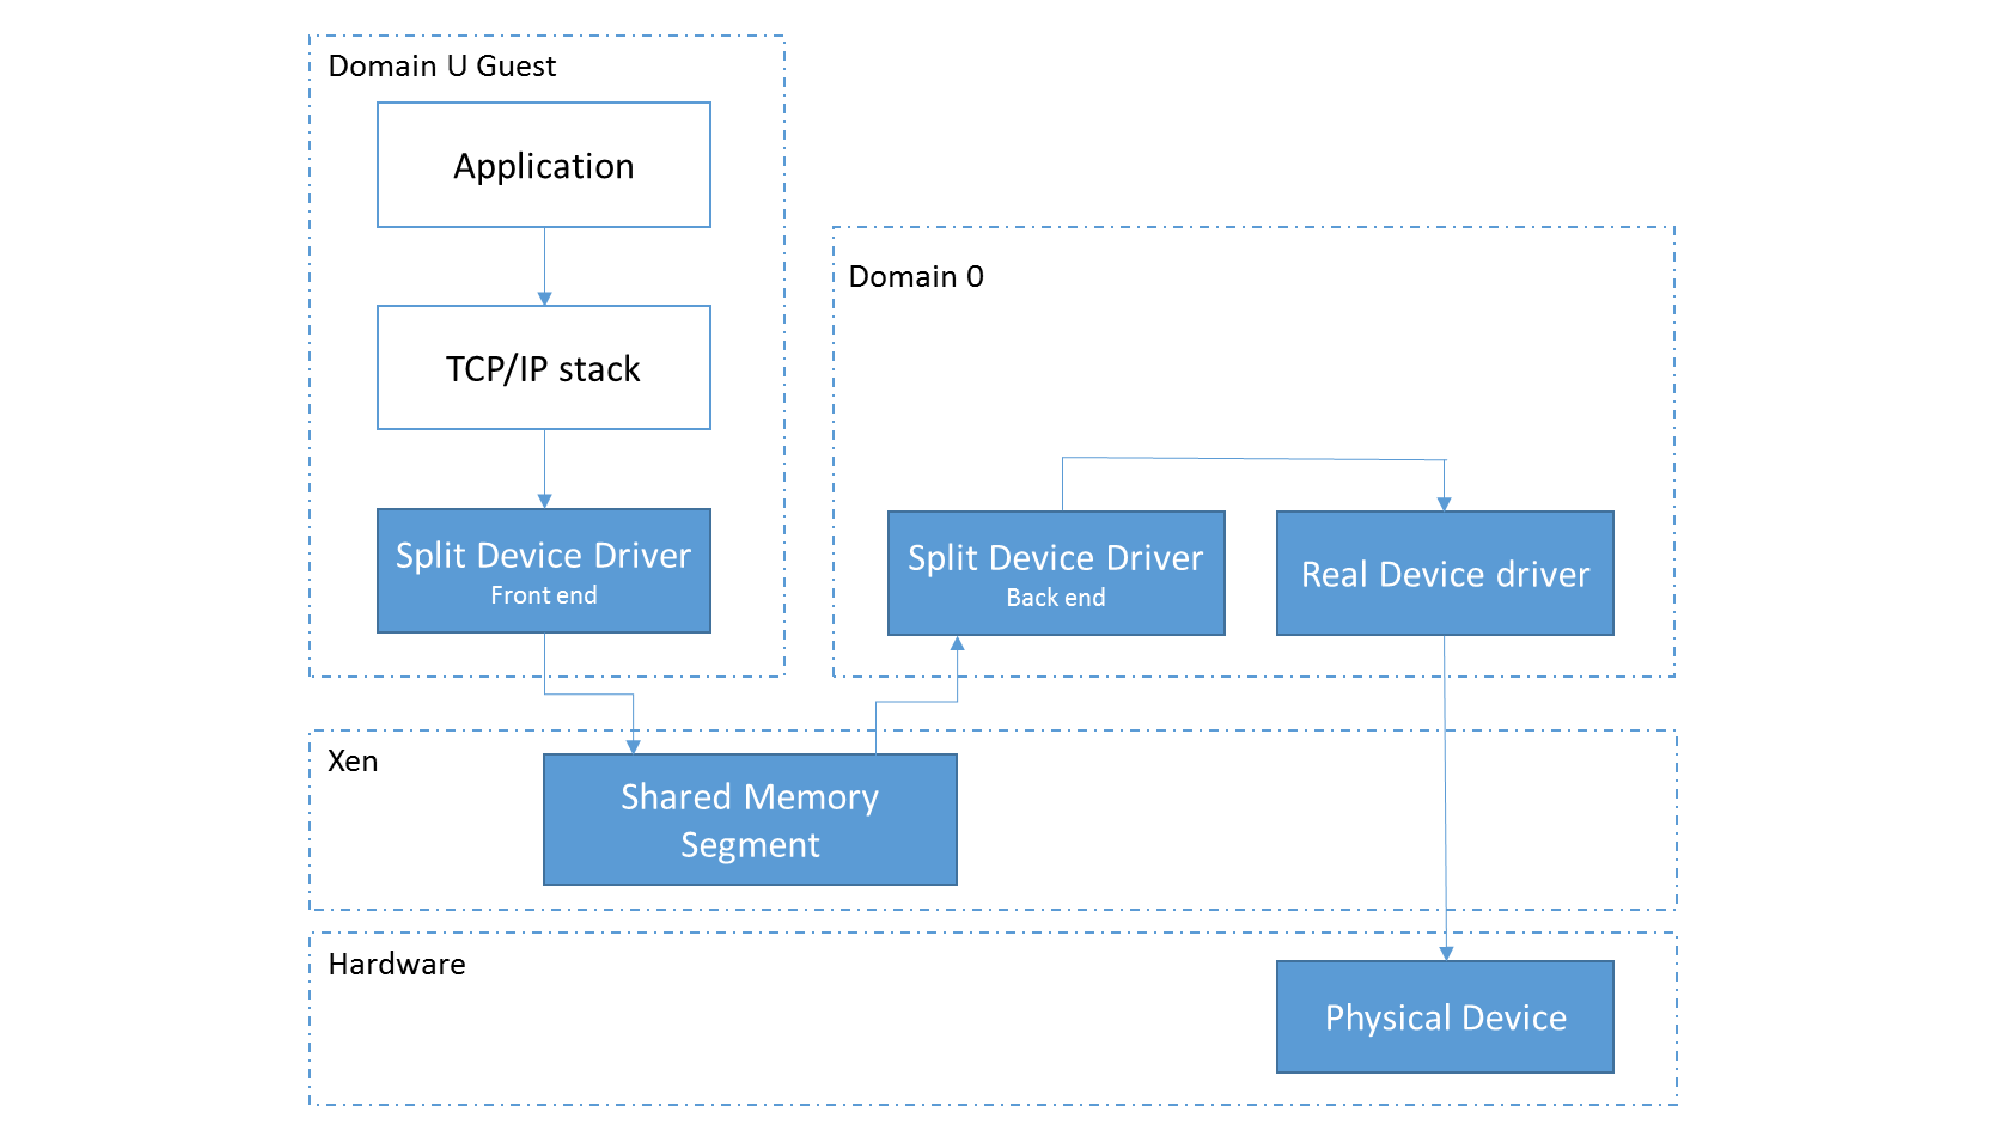
\includegraphics[scale=.50]{xen-split-tcp.pdf}
\caption{Split device driver model}
\label{fig:xen-split}
\end{figure}
Xen has a frontend driver in a domain U guest and a backend driver in the domain 0. The frontend and the backend driver transfer data between domains over a channel that is provided by the Xen VMM. Within the driver domain, the backend driver is used to demultiplex incoming data to the device and to multiplex outgoing data between the device and the guest domain~\cite{driverdomain}.
\\[3mm]
In the isolated driver domain system, user applications and a kernel are executed in a guest domain, and a device driver is executed in a driver domain. As a result, a device driver is isolated from the Linux kernel, making it impossible for the device driver to corrupt kernel data structures in the virtual machine running user applications. 
\\[3mm]
Despite advances in virtualization technology, the overhead of communication between guest and driver domains significantly affects the performance of applications~\cite{barham2003xen, Sugerman:2001:VID:647055.715774, Menon:2006:ONV:1267359.1267361}. Isolated driver domains follow an interrupt based approach for sending notifications~\cite{barham2003xen}. The frontend and backend notify each other of the receipt of a service request and corresponding responses by sending an interrupt. The Xen hypervisor needs to schedule the other domain to deliver the interrupt, which may require a context switch~\cite{barham2003xen}. Such context switches can cause system overhead~\cite{Li:2007:QCC:1281700.1281702, Mogul:1991:ECS:106973.106982}.

\section {Proposed Solution}
In this thesis, we propose and evaluate an optimization for improving the performance of the communication between guest and driver domains. We propose a solution in which a thread in the backend driver spins for some amount of time, checking for incoming service requests, and the frontend driver spins for some amount of time, checking for the responses. 
\\[3mm]
In uniprocessor and multiprocessor environment, a context switch takes a significant amount of time. In a multi-processor environment, it is more efficient for each process to keep its own CPU and spin while waiting for a resource~\cite{Bovet:2005:ULK:1077084}. Since our solution follows a spinning based approach, it performs better than the interrupt based approach used in the original implementation.
\\[3mm]
The source code of the isolated driver domain is not available in the open source Xen hypervisor code. In this thesis, we re-implement Xen's isolated driver domains, we refer to our implementation as Isolated Device Driver (IDDR). We then implement our spinning based optimization within IDDR.
\\[3mm]
The performance of the system is evaluated for multiple block device types, including ramdisks, loop devices, and SATA disks. A block device is formatted with a ext2 file system and the IDDR system is evaluated by measuring the performance of the system with SysBench benchmark. The integrity of the system is checked by executing reads and writes on a block device, with and without read ahead, file system tests on the variety of block devices. Our evaluation shows that the performance of the system can be improved by avoiding the context switches in the communication channel. The IDDR system trades off CPU cycles for the better performance. It uses CPU cycles spinning while waiting for requests and responses. Otherwise, these CPU cycles would have been used by an application.

\section{Core Contributions}
The core contributions of this project are listed below: 
\begin{enumerate}
\item Re-implementation of Xen's isolated driver domain - Isolated Device Driver (IDDR).
\item Improvement in the performance of the IDDR by implementing the spinning based communication channel instead of the interrupt based communication channel. 
\item A performance comparison of the spinning based IDDR and interrupt based IDDR.
\end{enumerate}
\section {Organization}
This section provides the organization and roadmap of the thesis.
\begin{enumerate}
\item Chapter 2 provides background on Processes, Threads, Memory Protection, Virtualization, Hypervisor and Inter-domain Communication.
\item Chapter 3 provides an introduction to design of the system to isolate device driver. 
\item Chapter 4 discusses the detailed design and implementation of IDDR. 
\item Chapter 5 evaluates the performance of IDDR.
\item Chapter 6 reviews related work in the area of kernel fault tolerance.
\item Chapter 7 concludes the thesis and lists possible topics where this work can be extended.
\end{enumerate}
\pagebreak
\ifbool{toShowBibliography}{\bibliography{references}}{}